\documentclass[11pt, oneside]{scrartcl}   	% use "amsart" instead of "article" for AMSLaTeX format
\usepackage{geometry}                		% See geometry.pdf to learn the layout options. There are lots.
\geometry{a4paper}                   		% ... or a4paper or a5paper or ... 

\usepackage{graphicx}				% Use pdf, png, jpg, or eps§ with pdflatex; use eps in DVI mode
								% TeX will automatically convert eps --> pdf in pdflatex		
\usepackage{amssymb}
\usepackage{listings}				% For code snippets
\usepackage{hyperref}				% For hyperlinks

%SetFonts

%SetFonts
\lstset{language=C} 

\title{Embedded Systems Exam Bonus Project}
\subtitle{Project name: Green Gardening}
\author{Contributers: Leander Lauenburg, Christoph Clement, Anselm Coogan}
\date{18.01.18}	

\begin{document}
\maketitle
\section{Hardware}

\subsection{\href{http://www.cypress.com/documentation/development-kitsboards/cy8ckit-042-psoc-4-pioneer-kit}{CY8CKIT-042 PSoC� 4 Pioneer Kit}}

Cypress' CY8CKIT-042 PSoC 4 Pioneer Kit is used as the basis for the project. We decided to use Cypress? product because of several reasons. First, the father of a team member works for Cypress and we got the Pioneer Kit for free which is always great. Second, Cypress' PSoC Creator Software to program the kit is a free IDE which features hardware and software co-design and a library with pre-characterized PSoC components. Third, Cypress offers the PSoC 101 Video Tutorial Series which demonstrates how to use the development kits. We all watched the videos and could learn a lot from them.

The kit contains the PSoC 4 Pioneer board, a quick start guide, a USB Standard-A to Mini-B cable and six jumper wires.

The Pioneer Kit consists of the following blocks:
\begin{itemize}
	\item PSoC 4
	\begin{itemize}
		\item 32-bit MCU subsystem, 48 MHz ARM Cortex-M0 CPU, 32 KB flash, 4 KB SRAM
		\item Programmable analog: Two opamps, 12-bit SAR ADC
		\item Low power 1.71 to 5.5 V operation
		\item Serial communication via I2C, SPO and UART
		\item Timing and pulse-width modulation 
	\end{itemize}
	\item PSoC 5LP
	\begin {itemize}
		\item used to program and debug PSoC 4
		\item 32-bit ARM Cortex-M3 CPU core
		\item Precision, programmable clocking: 32.768 kHz watch crystal oscillator
	\end{itemize}
	\item Power supply system
	\item PSoC 5LP GPIO header (J8)
	\item Programming interfaces (J6, J7, J10)
	\item CapSense slider
	\item Arduino compatible headers 
	\item Pioneer board LEDs
	\item Digilent Pmod compatible header (J5)
	\item Push buttons (Reset and User buttons)
\end{itemize}

\begin{figure}[htbp]
	\begin{center}
	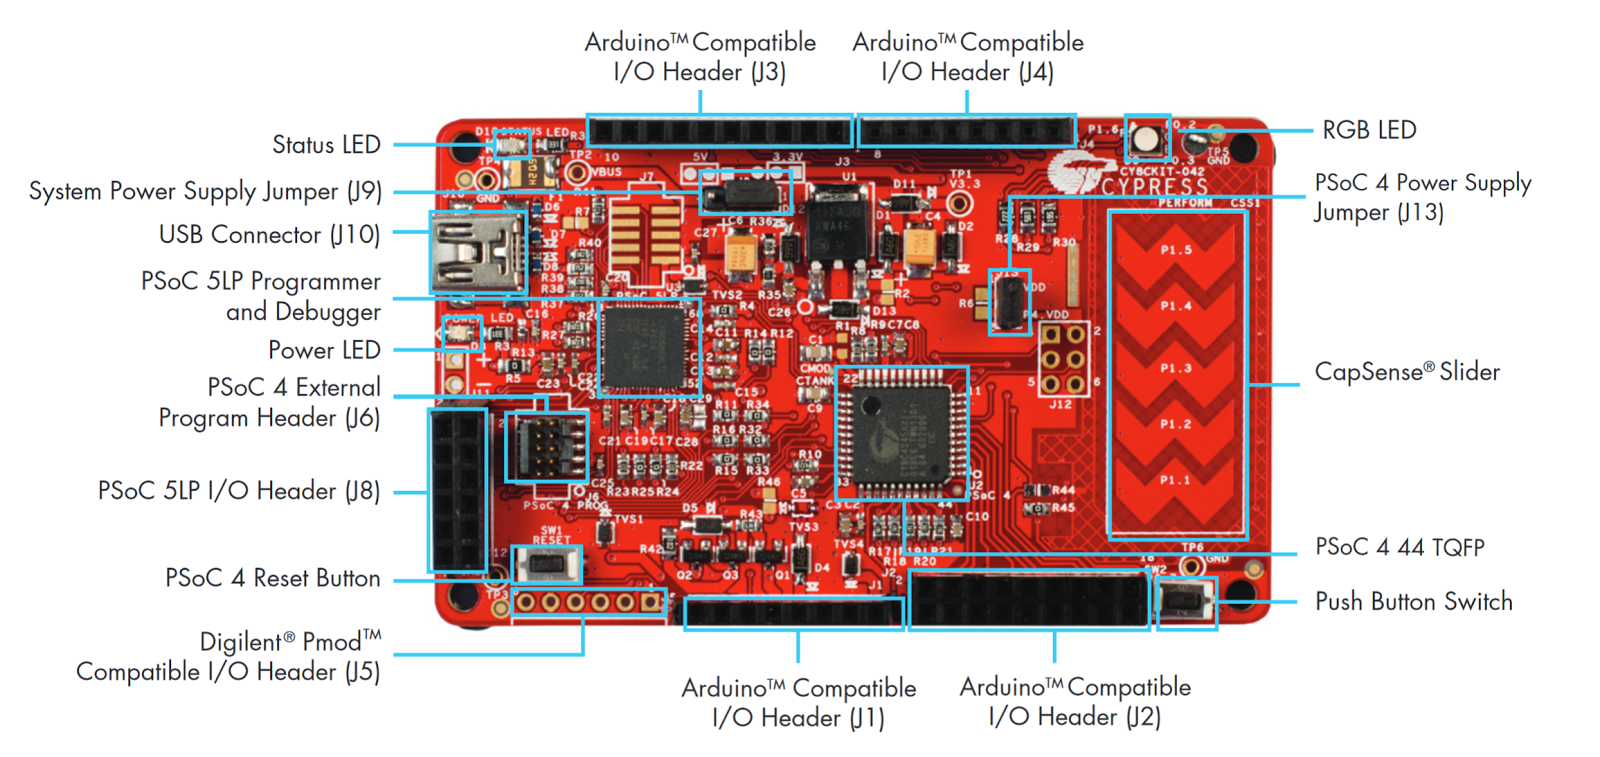
\includegraphics[width=\linewidth]{micro.png}
	\caption{PsoC 4 Pioneer Board}
	\label{fig:micro}
	\end{center}
\end{figure}

\subsection{Kuman moisture sensor}

The soil moisture module is used to detect the moisture content of the soil. If the soil is too dry the electrical pump is switched on. It is possible to adjust the threshold of the soil humidity with the potentiometer. The digital output D0 is directly connected to the pioneer kit via a digital input  pin. The operating voltage is 3.3 V to 5 V and is supplied from the pioneer kit.

\begin{figure}[htbp]
	\begin{center}
	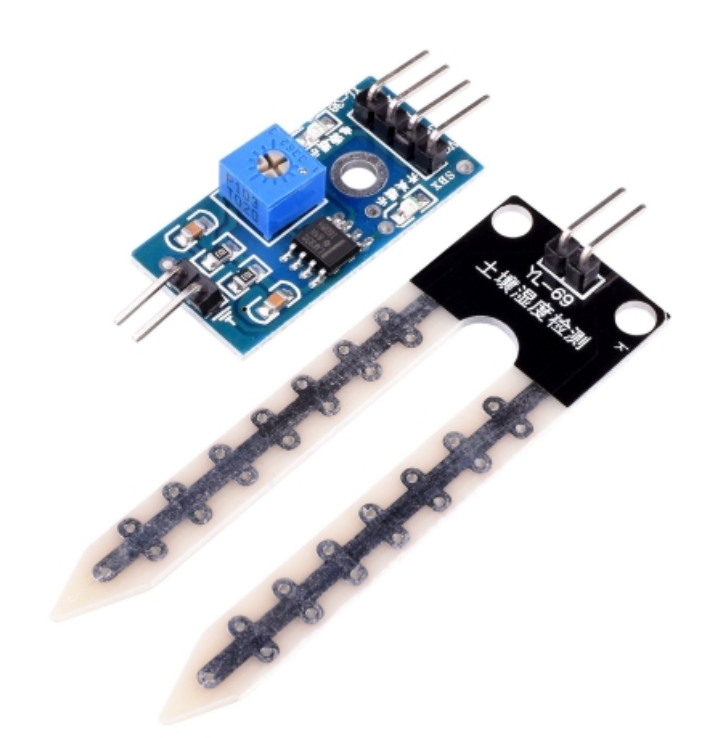
\includegraphics[width=50mm, scale=0.5]{moisture-sensor.png}
	\caption{Kuman moisture sensor}
	\label{fig:moisture}
	\end{center}
\end{figure}

\subsection{Arduino light sensor LM393}

The light sensor works pretty similar to the moisture sensor.  It detects the brightness of the surroundings. If there is not enough sunlight the LEDs are turned on. The threshold can be adjusted with the potentiometer. The digital output pin D0 is connected to the pioneer kit via a digital input pin. The operating voltage is 3.3 V to 5 V and is supplied from the pioneer kit.

\begin{figure}[htbp]
	\begin{center}
	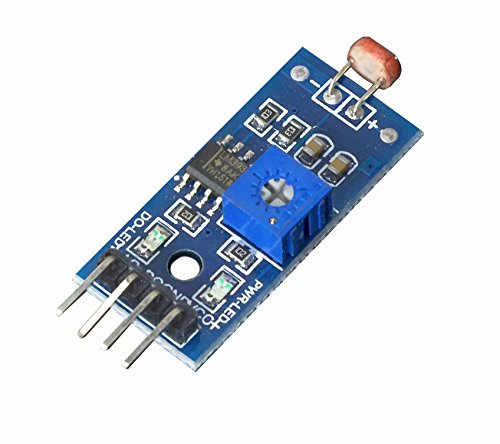
\includegraphics[width=50mm, scale=0.5]{light-sensor.png}
	\caption{Arduino light sensor LM393}
	\label{fig:moisture}
	\end{center}
\end{figure}

\subsection{LE Trafo 12V DC}

The 12V Trafo is used as a power supply for the LED stripes and brushless mini water pump. Its input voltage is 100-240 V AC, 50 - 60 Hz and output voltage 12 V DC, 2A.

\subsection{SainSmart 4 channel relay module}

The SainSmart relay module allows the PSoC to control larger loads and devices like the 12 V LED stripes and the brushless water pump with a digital output pin. The operating voltage is 5 V and each relay needs 15-20 mA driver current. 

\begin{figure}[htbp]
	\begin{center}
	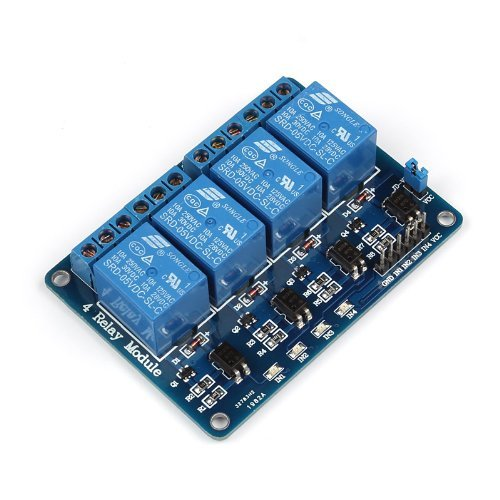
\includegraphics[width=50mm, scale=0.5]{relais.png}
	\caption{SainSmart 4 channel relay module}
	\label{fig:relais}
	\end{center}
\end{figure}

\subsection{TSSS brushless mini water pump}

The brushless mini water pump is switched on for 10 seconds via a digital output pin from the PSoC that controls the relay if the soil is too dry. It pumps water from a basket and moistures the soil. The operating voltage is 12 V and it needs 400 mA driver current. This is supplied by the 12 V Trafo.

\subsection{Neuftech LED strips blue and red}

The LED strips in blue and red work similar to the water pump. They are switched on via a digital output pin from the PSoC that controls the relay if there is not enough sunlight. The operating voltage is 12 V. This is supplied by the 12 V Trafo.

\subsection{Plant}

The most important part for our project: a nice plant that will hopefully survive for a long time with the help of all the other parts.

\subsection{Schematic}

TODO

\section{Software}

As stated in the previous chapter we used the free IDE \emph{PsoC Creator} to program the micro controller. This software offers a three layer approach. 

In the first layer, the top design, you can graphically configure the technical layout and wiring of the components you are using from the micro controller. In the second layer you assign the actual pins of the board to the different components configured in the top design. Lastly, the third layer is writing the code that is executed on the micro controller.

The entire source code discussed here (and successive versions) can be inspected in this git repository: https://github.com/AnselmC/GreenGardening

\subsection{Top design}

The top design enables you to easily make a circuit diagram for your project. You have access to all the actual components of the micro controller, as well as so-called off-board components that are there for documentation and clarification purposes only (colored blue). The components we used for this project are: a real-time clock, a universal asynchronous receiver transmitter, and digital input and output pins.

\subsubsection{Real-time clock}

The built-in real-time clock component can be configured extensively and has a resolution of one second. We set the clock to use the 24-hour time format and synched it to Central European Time.

\subsubsection{UART}

The universal asynchronous receiver transmitter component allows for setting up a bidirectional data connection on a given port. We are using this for debugging purposes. 

\subsubsection{Digital input pins}

The input pins in our project are the light sensor and the moisture sensor. We configured these input pins to have dedicated interrupts. The interrupt for the light sensor is activated on both falling and rising edges, i.e. from light to dark and vice versa. This is because the light sensor is situated so that it is independent of the LED strips and only senses the environment light. Thus, if the LED's have been switched on because it was previously too dark and now the surrounding light suffices the LED's should be switched off. In contrast the interrupt for the moisture sensor is only activated on a falling edge, i.e. when it gets too dry. 

\subsubsection{Digital output pins}

As output pins we have set up the water pump and the LED strips.

\subsection{Pin connections}

The second layer is actually called \emph{Design Wide Resources}. However, we are only using the pin assignment part in our project. Here you get an overview of the micro controller  and can then assign the components configured in the top design with the components on the board and the components that have been connected via the digital or analog GPIO pins.

\subsection{C Code}

PsoC Creator automatically generates an API from the top design previously configured. This allows you to control all components with very little self-written C code.
In our main.c we have defined the following global variables used throughout our code:

\begin{itemize}
	\item WATERING\_TIME\_IN\_SEC: the time the watering pump should be on for one watering session
	\item STARTING\_HOUR and ENDING\_HOUR: the timeframe in which the plant should be exposed to light - in 24 h format (e.g. from STARTING\_HOUR: 10 to ENDING\_HOUR 20)
	\item NUMBER\_OF\_MEASUREMENTS: The number of measurements a sensor should make in one setting
	\item TIME\_BETWEEN\_MEASUREMENTS\_MILSEC: The time (in milliseconds) to wait between the single measurements
	\item BUFFER\_SIZE: The array size of the buffer used for writing debug information to the console
	\item ON and OFF: Macros used for more clarity in code
\end{itemize}

In order to use less CPU time and power, we are working with interrupts. There are two interrupts: one for the moisture sensor and one for the light sensor. The interrupts are triggered on both falling and rising edges of the sensors. This means that whenever the light changes from too dark to light or vice versa, or the moisture sensor changes from not moist enough to moist and vice versa the interrupts are called. In PsoC Creator these interrupts are configured in main.c as follows (for an arbitrary pin named Pin\_A):

\begin{lstlisting} [frame=single]
CY_ISR(<<name_of_interrupt_handler>>)
{
    /* Code to be executed on interrupt */
    
    Pin_A_ClearInterrupt();
}
\end{lstlisting}

The name of the interrupt handler can be whatever you choose. However, best practice is to name it \emph{Pin\_A\_Handler}. It is essential to clear the interrupt after the code has been executed, otherwise the interrupt can?t be called again. This is done with the generated \emph{Pin\_A\_ClearInterrupt()} function. In order to enable interrupt handling, in your \emph{main()} method you will need to call \emph{CyGlobalIntEnable}. Then, you need to initialize every interrupt like this: \emph{Pin\_A\_int\_StartEx(Pin\_A\_Handler)}
The StartEx function of your interrupt-enabled pin is also automatically generated by PsoC Creator. This means that in our project the \emph{main()} function solely consists of initializing the interrupts and an endless for-loop with no-code. Thus, the CPU can sleep until one of the sensors interrupts it. 

\begin{lstlisting}[frame=single]
int main(void)
{
    /* Enable global interrupts. */   
    CyGlobalIntEnable; 

    /* Place initialization/startup code here */
    UART_Start();
    RTC_Start();
    Pin_Light_Sensor_int_StartEx(Pin_Light_Sensor_Handler);
    Pin_Moisture_Sensor_int_StartEx(Pin_Moisture_Sensor_Handler);
    
    for(;;)
    {
        
    }
}
\end{lstlisting}

Our two interrupt functions each call one function, namely \emph{checkLight()} and \emph{checkMoisture()}.
\emph{checkLight()} first calls the real-time clock component to return the current time and then extracts the current hour. It then checks whether the returned hour is in the designated timeframe. If it isn't, the light is turned off and the function terminates. If it is, then we take a pre-defined amount of measurements (as configured in the global variables) with a pre-defined delay between each measurement. If the light sensor only measures enough light for less than half of the measurements, the LED's are turned on and the function terminates. Else, the lights are turned off and the function terminates.

\begin{lstlisting} [frame=single]
void checkLight()
{
    /* Get current hour */
    int hour = RTC_GetHours(RTC_GetTime());
    
    /* Check whether hour is outside of designated time frame 
    if so, turn it off */
    if(hour < STARTING_HOUR || hour > ENDING_HOUR){
        Pin_LED_blue_Write(OFF);
    }
    else {
        int positive_measurements = NUMBER_OF_MEASUREMENTS;
        /* Make several measurements of the light sensor */
        for(int i = 0; i < NUMBER_OF_MEASUREMENTS; i++){
            positive_measurements -= Pin_Light_Sensor_Read();
            CyDelay(TIME_BETWEEN_MEASUREMENTS_IN_MILSEC);
        }
        /* If the light sensor catches not enough light, 
        turn on the LED's */
        if (positive_measurements < NUMBER_OF_MEASUREMENTS/2)
        {
            Pin_LED_blue_Write(ON);   
        } 
        /* Else turn them off */
        else 
        {
            Pin_LED_blue_Write(OFF);
        }
    }
}
\end{lstlisting}

The \emph{checkMoisture()} function operates similarly. Again, we take a pre-defined amount of measurement to rule out anomalies. Then, if less than half of these measurements indicate that the soil is too dry, the water pump is turned on for a specified amount of time and then turned off again after which the function terminates. If the soil is moist enough, nothing happens and the function terminates.
\begin{lstlisting}[frame=single]
void checkMoisture()
{
    int positive_measurements = NUMBER_OF_MEASUREMENTS;
    /* Make several measurements of the moisture sensor */
    for(int i = 0; i < NUMBER_OF_MEASUREMENTS; i++){
        positive_measurements -= Pin_Moisture_Sensor_Read();
        CyDelay(TIME_BETWEEN_MEASUREMENTS_IN_MILSEC);
    }

    /* If the ground isn't wet enough, 
    water the plant for a specified amount of time */
    if (positive_measurements < NUMBER_OF_MEASUREMENTS/2)
    {
        /* Turn pump on */
        Pin_pump_Write(ON);
        /* Wait for specified amount of watering time */
        CyDelay(WATERING_TIME_IN_SEC * 1000);
        /* Turn pump off */
        Pin_pump_Write(OFF);
    }
}
\end{lstlisting}

Throughout the code we are outputting debug information that was critical for development. For this we are using the UART component. To use it it must be be initialized in the \emph{main()} method as can be seen above. Then, when you want to write to the connected pod (e.g. a terminal on your development machine) you can do so like this:

\begin{lstlisting}[frame=single]
sprintf(buffer, "Let's go\r\n");
UART_UartPutString(buffer);
\end{lstlisting}

\section{Learnings from the lecture}

The lecture related to is a union of the two lectures Embedded Systems and Real Time Systems, as they are closely related. How strong these two subject interleave became as much clearer while releasing this Project.

\subsection{The System}
  
According to the lecture an embedded system is a system which has a particular function within a larger mechanical or electrical system, often with real-time computing constraints. 
It is therefore quite far-fatched to call the Modul in use embedded.  The Modul is the only and therefore main logic in our system and most definitely isn't the system a ?larger? mechanical system.
But since the system does has real-time computing constraints and the System is just in the making, expecting expansion through hardware and additional logic parts in the near future, it will from her on be referred to as an Embedded System.
However at this moment the system is a synchronous digital circuit since ?all? logic is connected to the same clock.
A real-time System is defined as a computer system which accuracy doesn?t only depend on the logical result but also on the physical point in time by which the result is produced. 
 
Since certain tasks of our system depend on the time of the day it has to be referred to as ?real-time System? according to this definition, also the author probably had a bit smaller unit for the time in mind.
At the moment we are working on extending the systems functionality by making use of the PSoC?s integrated Bluetooth interface. Thereby transforming the system to a smart device making it controllable via smartphone as well as graphically representing the accumulating data on the phone.
By doing so the system will become a Cyber-physical systems in accordance with the definition of Cyber-physical systems from the lecture.

\subsection{Operator Cluster}

The human who makes use of the system, calibrating it to the specifics of the plant and turning the system on and off.

\subsection{Computational Cluster}

The \_\_\_\_\_ Modul from Cypress.
 
\subsection{Controlled Cluster}

Is made up of the sensors as well as the light and the pump.

\subsection{The Logic}
Since ?embedded System? refers to how a logic device is integrated in a larger system and not the device itself it can refer to just about every logic device. 
All these different devices were categorized in the lecture.
The module in use (for more information on the model refer to the hardware chapter) is an ?Programmable System on a Chip? (PSoC).
We choose the module inspired by a reference from the lecture referring to its great flexibility as well as great compatibility. 
Additionally we were really keen on trying out the IDE PSoC creator which was also referred to in the lecture.
At the beginning of our project we sat down analysing the module with the information given to us by the lecture. 
We recognised the real time capability of the ARM Cortex-M0 CPU through characteristic like the on board real time clock supported by an on board button cell and the by default missing cache. 
From the lecture we knew that also most of the time a cache increases the performance of the device it can in extreme cases lead to a greater worst case runtime making timing issues difficult to analyse. 
\subsection{Real time}
As stated already in the beginning of this chapter the System can be categorized as a real time system. This is at moment manly do to the implementation of the lighting system.    
The implementation of the lighting system as it is is a combination of a ?Time triggered applications? and an ?Event-driven applications?. The light is supposed to switch on whenever the light sensor signals that it is to dark. Therefore it is clearly event driven. 
But since a plant naturally also needs a time during which it is dark the signal of the light sensor should only be incorporate during certain times of the day. In the extreme case of permanent total darkness the light will always be switch on over a constant time period during a certain time of the day. In this case you can without objection say that the entire time cycle was determined during compile time thereby making it a pure time triggered application. 
It would be possible to realise the system through purely time triggered applications. But this would lead to an reduction in flexibility and effectiveness of the system since parameters for temperature and humidity would have to be known already during compile time. These parameters would also have to be final since time triggered applications by definition don?t react to external signals and are therefore inflexible. 
The dependency on the time of the day is what makes the system a real time system.
Thanks to an on board real time clock the modul can guarantee the accuracy of the system. A button cell powers the clock during times in which the modul isn?t connected to its main power supply, for example during transport.   
It would be preferable to use an mor accurate external quartz crystal oscillators to minimize the drift.  
But since most plants are quite durable the don't require such high precision for when the light shines and when not.
This leads directly to the question of what kind of real time system we are dealing with.
For hard real time systems the lecture states:
 
?A violation of the defined deadlines can immediately lead to severe consequences?
 
A plant pretty much doesn't care when it is watered and at what time of the day it gets light as long as it gets enough of both in the end of the day. 
Therefore if the system fails to react instantaneously to a signal of one of the sensors or the clock there won't be any severe consequences.
For soft real time systems the lecture states among other things: 
?...an overrun of those deadlines is not catastrophic...?
and
?Overall it is possible that the breach of the time limit will produce a degradation in service...?
The system is therefore clearly a soft real time system. Since a miss of a deadline can in the worst case only result in a degradation of growth of the plant. 


\end{document}  